\documentclass{article}

\usepackage[margin=1in]{geometry}
\usepackage[T1]{fontenc}
\usepackage[utf8]{inputenc}
\usepackage{lmodern}
\usepackage{amsmath,amssymb}
\usepackage{graphicx}
\usepackage{xcolor}
\usepackage{hyperref}
\usepackage{listings}
\usepackage{booktabs}
\usepackage{array}
\usepackage{longtable}
\usepackage{float}
\usepackage{enumitem}
\usepackage{tikz}
\usetikzlibrary{arrows.meta,positioning,fit,calc,shapes.geometric}

\hypersetup{
  colorlinks=true,
  linkcolor=blue!60!black,
  urlcolor=blue!60!black
}

\definecolor{codebg}{RGB}{248,248,248}
\definecolor{codecomment}{RGB}{0,110,80}
\definecolor{codekeyword}{RGB}{0,70,140}
\definecolor{codestring}{RGB}{163,21,21}

\lstdefinestyle{code}{
  backgroundcolor=\color{codebg},
  basicstyle=\ttfamily\small,
  commentstyle=\color{codecomment},
  keywordstyle=\color{codekeyword}\bfseries,
  stringstyle=\color{codestring},
  showstringspaces=false,
  breaklines=true,
  frame=single,
  rulecolor=\color{black!20},
  tabsize=4,
  keepspaces=true,
  captionpos=b
}

\newcolumntype{L}[1]{>{\raggedright\arraybackslash}p{#1}}
\setlist[itemize]{leftmargin=1.5em}

\tikzset{
  diagbox/.style={
    draw,
    rounded corners=2pt,
    thick,
    fill=blue!6,
    align=center,
    inner sep=5pt,
    minimum height=9mm,
    font=\small
  },
  processbox/.style={diagbox, fill=blue!8},
  storebox/.style={diagbox, fill=orange!10},
  artifactbox/.style={diagbox, dashed, fill=green!8},
  groupbox/.style={draw, dashed, rounded corners=4pt, inner sep=7pt},
  flow/.style={-Latex, thick},
  genflow/.style={-Latex, thick, dotted}
}

\title{AI Sports Agent via LLM Tool Planning and Probabilistic Model Checking\\
\large A Source-Code Analysis of the AI Badminton Coach}
\author{}
\date{April 19, 2026}

\begin{document}
\maketitle

\section{Abstract}
This report analyzes the complete source code of an AI sports-agent project whose concrete implementation is an \emph{AI Badminton Coach}. The system operationalizes a principled division of labor between a large language model and a formal verification engine: the LLM is restricted to planning and explanation, while match-winning probabilities are computed externally through a parametric PCSP\# model executed by PAT Console or, in development mode, by a deterministic mock verifier. The repository contains a full pipeline for player resolution, historical feature extraction, schema-enriched ShuttleSet ETL, calibrated probability construction, strategy perturbation, backtesting, and artifact generation. The shipped dataset contains 27 players and 44 matches, and the codebase is supported by 66 passing automated tests, a leakage-aware time-machine backtesting harness, CLI and FastAPI interfaces, and auditable run directories that preserve rendered models, parameters, PAT outputs, and summaries. The overarching result is an inspectable architecture in which natural-language interaction is retained, but the numerically critical reasoning path is moved into typed Python parameterization and formal model-checking machinery.

\section{Introduction}
Probabilistic model checking (PMC) provides a mathematically explicit way to evaluate stochastic systems. Instead of asking a language model to estimate a probability directly, PMC encodes the system as a state-transition process with probabilistic branches and then evaluates temporal or reachability properties over that process. In this repository, PAT is the execution engine and PCSP\# is the modeling language used to express badminton match dynamics.

This design responds to a fundamental weakness of ordinary LLM-only sports assistants. A pure LLM can describe strategy fluently, but it has no internal guarantee that its numbers correspond to a coherent stochastic process. Numerical outputs may be hallucinated, inconsistent across turns, or disconnected from the actual structure of a match. These limitations are especially serious when the task is not mere text generation, but a claim such as ``Player A has a \(49.8\%\) chance to win'' or ``a \(3\%\) increase in short-serve frequency improves winning odds by \(1.5\) percentage points.''

The codebase addresses this problem by turning the LLM into a \emph{tool-using planner} rather than a calculator. The current implementation does \emph{not} let the LLM generate arbitrary PCSP\# syntax token by token. Instead, the LLM is constrained to produce typed JSON plans, after which deterministic Python code resolves players, computes features from historical data, injects parameters into a generic PCSP\# template, runs PAT, and finally summarizes the computed result. The repository therefore instantiates a broader ``AI Sports Agent'' concept with a badminton-specific case study that is technically rigorous and directly auditable.

\subsection*{Concrete Contributions of the Repository}
The repository makes several concrete contributions that are stronger than a generic ``LLM plus simulator'' design. First, it uses typed LLM-to-tool planning rather than free-form code or model generation, which sharply narrows the space for hallucinated execution. Second, it implements a ShuttleSet-to-match ETL pipeline that converts stroke-level badminton logs into an enriched historical schema suitable for downstream inference. Third, it couples a calibrated upstream parameterization layer with a downstream formal reachability model, so that rich historical features can influence prediction without requiring the language model to manipulate the formal system directly. Fourth, it provides a leakage-aware walk-forward evaluation harness with explicit point-in-time snapshots, baseline comparisons, and probability calibration. Fifth, it preserves full run artifacts, which makes the system inspectable as a research object rather than only as an interactive demo.

\section{System Architecture}
The repository is organized as a layered tool-using system rather than a monolithic chatbot. The control surfaces are \path{main.py}, \path{coach/cli.py}, and \path{coach/ui/app.py}; the planning layer lives in \path{coach/agent}; the data and model layers live in \path{coach/data} and \path{coach/model}; PAT integration lives in \path{coach/pat}; and evaluation and experimentation are implemented in \path{coach/analysis} and \path{coach/backtest}.

\begin{table}[H]
\centering
\small
\begin{tabular}{L{0.25\linewidth}L{0.69\linewidth}}
\toprule
Repository slice & Responsibility \\
\midrule
\path{coach/agent} & Prompt engineering, Gemini client, JSON schemas, planning logic, heuristic fallback, and natural-language result synthesis. \\
\path{coach/data} & Local CSV adapter, ShuttleSet-derived schema, player lookup, feature estimation, cold-start priors, head-to-head blending, and influence-weight fitting. \\
\path{coach/model} & Typed parameter validation, effective rally-probability computation, template rendering, and traceable parameter export. \\
\path{coach/pat} & Real PAT execution, mock execution for CI, text-output parsing, and PAT3-on-Mono compatibility handling. \\
\path{coach/service.py} & End-to-end orchestration for prediction and strategy optimization. \\
\path{coach/analysis} & Batch prediction, batch strategy, experiment orchestration, and plotting. \\
\path{coach/backtest} & Leakage-safe walk-forward evaluation, calibration, baseline models, and feature-contract export. \\
\path{scripts} & ShuttleSet ETL, PAT connectivity checks, inference-threshold validation, LLM smoke tests, and Redis key-management utilities. \\
\bottomrule
\end{tabular}
\end{table}

The end-to-end workflow is as follows:

\begin{itemize}
\item A user submits a query through the CLI, chat interface, or FastAPI endpoint.
\item The planner classifies the task as either \texttt{prediction/reachability} or \texttt{strategy/sensitivity}.
\item The executor resolves the player names against the local player table and loads historical statistics from the local CSV adapter.
\item \texttt{build\_matchup\_params()} converts those historical statistics into validated \texttt{MatchupParams}, including serve, receive, style, error, clutch, serve-type, stroke-profile, handedness, reliability, recent-form, and rest features.
\item \texttt{build\_matchup\_model()} injects those parameters into a generic PCSP\# template and writes both the rendered \path{matchup.pcsp} file and an auditable \path{params.json}.
\item \texttt{run\_pat()} executes PAT in real mode or a deterministic surrogate in mock mode.
\item The PAT text output is parsed, packaged into run artifacts such as \path{inputs.json}, \path{stats.json}, \path{summary.json}, and stdout/stderr logs, and summarized back into coaching language.
\end{itemize}

Figure~\ref{fig:end_to_end_pipeline} compresses that end-to-end story into one visual path. The abstraction is deliberately software-centric rather than UI-centric: the goal is to show where planning stops, where deterministic Python begins, and where the formal or mock verification step sits. Detailed schemas and parameter semantics are still unpacked in later sections.

\begin{figure}[H]
\centering
\resizebox{\linewidth}{!}{%
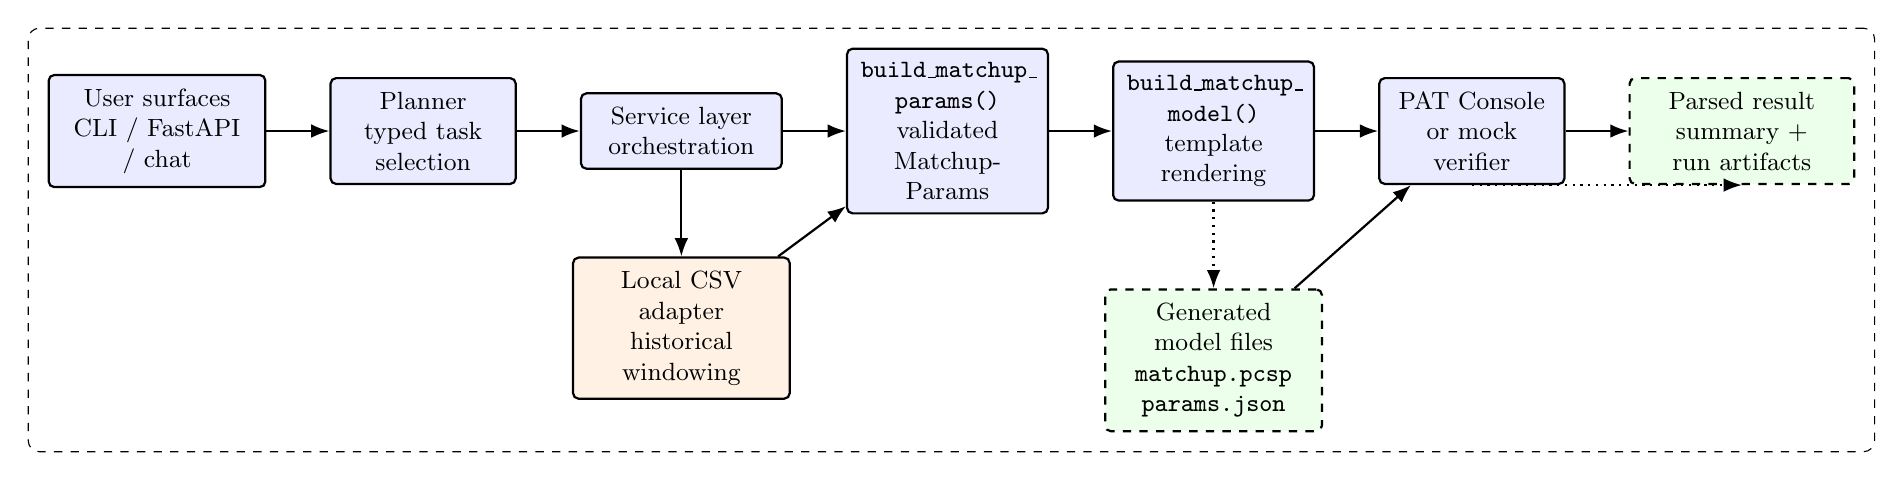
\begin{tikzpicture}[
  node distance=11mm and 8mm,
  every node/.style={font=\small}
]
\node[processbox, text width=2.4cm] (user) {User surfaces\\CLI / FastAPI / chat};
\node[processbox, right=of user, text width=2.0cm] (planner) {Planner\\typed task selection};
\node[processbox, right=of planner, text width=2.2cm] (service) {Service layer\\orchestration};
\node[storebox, below=of service, text width=2.4cm] (adapter) {Local CSV adapter\\historical windowing};
\node[processbox, right=of service, text width=2.2cm] (params) {\texttt{build\_matchup\_}\\\texttt{params()}\\validated MatchupParams};
\node[processbox, right=of params, text width=2.2cm] (model) {\texttt{build\_matchup\_}\\\texttt{model()}\\template rendering};
\node[artifactbox, below=of model, text width=2.4cm] (pcsp) {Generated model files\\\texttt{matchup.pcsp}\\\texttt{params.json}};
\node[processbox, right=of model, text width=2.0cm] (pat) {PAT Console\\or mock verifier};
\node[artifactbox, right=of pat, text width=2.5cm] (result) {Parsed result\\summary + run artifacts};

\draw[flow] (user) -- (planner);
\draw[flow] (planner) -- (service);
\draw[flow] (service) -- (params);
\draw[flow] (params) -- (model);
\draw[flow] (model) -- (pat);
\draw[flow] (pat) -- (result);
\draw[flow] (service) -- (adapter);
\draw[flow] (adapter) -- (params);
\draw[genflow] (model) -- (pcsp);
\draw[flow] (pcsp) -- (pat);
\draw[genflow] (pat) |- (result.south);

\node[groupbox, fit=(user)(planner)(service)(adapter)(params)(model)(pcsp)(pat)(result)] {};
\end{tikzpicture}
}
\caption{End-to-end AI Badminton Coach pipeline from user request to formal-model execution and auditable outputs.}
\label{fig:end_to_end_pipeline}
\end{figure}

A subtle but important implementation detail is that the LLM plan is \emph{advisory and typed}, not sovereign. In \path{coach/agent/planner.py}, the plan is validated against a Pydantic schema, but \texttt{AgentExecutor.run()} does not literally interpret arbitrary tool strings from a model response. Instead, it uses the validated task type to call deterministic service methods. This sharply limits the scope for hallucinated execution steps.

\begin{lstlisting}[style=code,language=Python,caption={Schema-constrained tool plan emitted for prediction queries in \texttt{coach/agent/planner.py}.}]
tool_calls = [
    ToolInstruction(tool="ResolvePlayers", arguments={"names": players}),
    ToolInstruction(
        tool="LoadStats",
        arguments={
            "playerA_id": "$playerA_id",
            "playerB_id": "$playerB_id",
            "window": window,
            "source": "local",
        },
    ),
    ToolInstruction(
        tool="BuildModel",
        arguments={
            "params": "$params",
            "template_name": "badminton_rally_template.pcsp",
            "out_path": "$run_dir/matchup.pcsp",
        },
    ),
    ToolInstruction(
        tool="RunPAT",
        arguments={
            "pcsp_path": "$pcsp_path",
            "pat_path": None,
            "mode": mode,
            "timeout_s": 60,
        },
    ),
    ToolInstruction(
        tool="SummarizeResults",
        arguments={
            "pat_outputs": "$pat_outputs",
            "question": user_query,
            "constraints": constraints,
        },
    ),
]
\end{lstlisting}

\section{Part A: The Parametric Formal Model}
The formal core of the repository is the template \path{coach/model/templates/badminton_rally_template.pcsp}. This file is explicitly designed as an \emph{injectable parametric model} rather than a matchup-specific script. No player-specific constants are hardcoded into the transition structure. Instead, all data-dependent quantities are inserted through placeholders such as \texttt{\{\{pA\_srv\_win\_w\}\}}, \texttt{\{\{serve\_mix\_A\_short\}\}}, and \texttt{\{\{target\}\}}.

The transition from raw data to PAT-ready integers occurs in \path{coach/model/params.py}. The class \texttt{MatchupParams} computes effective rally probabilities through a structured combination of baseline serve/receive skill, style differentials, error proxies, return pressure, clutch performance, serve-type effectiveness, rally tolerance, stroke-profile effects, handedness, reliability, recent form, and rest. The important modeling distinction is that the \emph{checked-in PCSP template remains intentionally compact}: it is still a serve/receive match automaton with a small number of probabilistic branches. The richer tactical information is currently injected \emph{upstream} into the effective probabilities computed in Python rather than represented as separate explicit PAT states. This design keeps the formal process graph manageable while still allowing the matchup parameters to be data-rich and auditable.

A simplified reading of the implementation is:
\[
\Delta_{\text{style}} =
w_{\text{short}}(s_A-s_B) +
w_{\text{attack}}(a_A-a_B) -
w_{\text{safe}}(\sigma_B-\sigma_A),
\]
and then
\[
p^{\text{srv}}_A = \operatorname{clamp}(\tilde{p}^{\text{srv}}_A + \Delta_{\text{serve}}),
\qquad
p^{\text{rcv}}_A = \operatorname{clamp}(\tilde{p}^{\text{rcv}}_A + \Delta_{\text{receive}}),
\]
where \(\tilde{p}\) is a reliability-weighted blend of player \(A\)'s own baseline and the complement of player \(B\)'s corresponding phase baseline. The full code further attenuates some features differently on serve and receive phases through fixed scale coefficients.

An additional implementation detail that matters for interpretation is that the parameterization is \emph{phase-asymmetric}. In \texttt{effective\_probabilities()}, the serve-side and receive-side deltas are not computed by reusing one common formula. Return pressure, serve-type effectiveness, rally tolerance, error profile, handedness, backhand usage, around-the-head usage, recent form, and rest are all scaled differently depending on whether the phase is own-serve or own-receive. Moreover, the newer micro-features are reliability-gated through the minimum of the two players' reliability values, so sparse historical evidence deliberately suppresses the impact of more speculative matchup edges. This means the code is doing more than a single undifferentiated ``feature sum'': it is encoding a cautious prior that some tactical signals should matter less when sample support is weak and that some signals should manifest differently across serve and receive contexts.

Because PAT's \texttt{pcase} branches are encoded as integer weights, the floating probabilities are scaled by \(10{,}000\) before template injection.

\begin{lstlisting}[style=code,language=Python,caption={Probability-to-weight translation in \texttt{coach/model/params.py}.}]
eff = self.effective_probabilities()
scale = 10000

p_a_srv_w = int(round(eff["pA_srv_win"] * scale))
p_a_rcv_w = int(round(eff["pA_rcv_win"] * scale))

context = {
    "target": self.target,
    "cap": self.cap,
    "best_of": self.best_of,
    "games_to_win": (self.best_of // 2) + 1,
    "pA_srv_win": f"{eff['pA_srv_win']:.6f}",
    "pA_rcv_win": f"{eff['pA_rcv_win']:.6f}",
    "pA_srv_win_w": p_a_srv_w,
    "pA_srv_lose_w": scale - p_a_srv_w,
    "pA_rcv_win_w": p_a_rcv_w,
    "pA_rcv_lose_w": scale - p_a_rcv_w,
}
\end{lstlisting}

The rendered PCSP\# model itself is compact. It tracks games, points, and current server; uses best-of-3 rules with target 21 and cap 30; and asserts the probability that player \(A\) reaches the winning terminal condition.

\begin{lstlisting}[style=code,language=C,caption={Core of the parametric PCSP\# template in \texttt{coach/model/templates/badminton\_rally\_template.pcsp}.}]
#define TARGET {{target}};
#define CAP {{cap}};
#define GAMES_TO_WIN {{games_to_win}};

enum{A, B};

var a_games = 0;
var b_games = 0;
var a_points = 0;
var b_points = 0;
var server = A;

#define A_GameWin ((a_points >= TARGET && (a_points - b_points) >= 2) || a_points == CAP);
#define B_GameWin ((b_points >= TARGET && (b_points - a_points) >= 2) || b_points == CAP);

BadmintonMatch = Rally;

Rally = [a_games < GAMES_TO_WIN && b_games < GAMES_TO_WIN]
    ([server == A] ServeA [] [server == B] ServeB);

ServeA = pcase {
    {{pA_srv_win_w}}: AWinServe -> UpdateA
    {{pA_srv_lose_w}}: BWinOnA -> UpdateB
};

ServeB = pcase {
    {{pA_rcv_win_w}}: AWinReceive -> UpdateA
    {{pA_rcv_lose_w}}: BWinServe -> UpdateB
};

#define A_WinsMatch a_games == GAMES_TO_WIN;
#assert BadmintonMatch reaches A_WinsMatch with prob;
\end{lstlisting}

\subsection*{A Concrete Execution Path Through the PCSP\# Automaton}
It is also useful to read the checked property operationally rather than only symbolically. Suppose the current state has \texttt{server == A}. Control enters \texttt{ServeA}, where a probabilistic branch is chosen according to the injected integer weights \texttt{pA\_srv\_win\_w} and \texttt{pA\_srv\_lose\_w}. If player \(A\) wins the rally, the process takes the \texttt{AWinServe -> UpdateA} branch; \texttt{UpdateA} increments \texttt{a\_points} and leaves the server as \(A\), which matches rally-point badminton scoring in which the rally winner serves next. If player \(A\) loses the rally, execution takes \texttt{BWinOnA -> UpdateB}; \texttt{UpdateB} increments \texttt{b\_points} and switches the server to \(B\). The same logic holds symmetrically in \texttt{ServeB}, except that player \(A\)'s rally success there is interpreted as a receive-side point and therefore governed by \texttt{pA\_rcv\_win\_w}.

After each point update, control moves to \texttt{CheckGame}. If neither \texttt{A\_GameWin} nor \texttt{B\_GameWin} holds, the process returns to \texttt{Rally} and the next point is simulated from the updated server state. If one side has won the game, the appropriate end-game transition increments the game counter, resets both point counters to zero, and sets the next server to the game winner. \texttt{NextState} then either starts the next game or terminates the match if one side has reached \texttt{GAMES\_TO\_WIN}. The reachability assertion therefore corresponds exactly to the coaching question: over all stochastic point-by-point continuations of this best-of-three rally process, what is the probability that player \(A\) reaches the winning terminal state first?

This walkthrough matters because it clarifies that the formal model is not merely a static probability container. It is a small but complete stochastic program over points, games, and server possession. The probability reported by PAT is therefore a match-level consequence of repeated rally-level branching under badminton scoring rules, not just a direct restatement of the input serve/receive probabilities.

This design is the crucial bridge between LLM interaction and formal verification. The LLM never writes this process graph directly. Instead, it selects a task, while Python deterministically instantiates a validated stochastic model.

\subsection*{What the Formal Engine Actually Sees}
It is useful to state more explicitly what is and is not inside the formally checked model. The rendered \path{matchup.pcsp} file includes a long comment header containing traceability fields such as player names, effective probabilities, tactical knobs, stroke-profile rates, handedness flags, reliability values, and fitted weights. These values are indeed exported into the template context and written into the concrete \path{.pcsp} file, but the PAT-executed state machine only uses a strict subset of them as operative semantics. Concretely, the formal transition structure depends on the match-format constants \texttt{TARGET}, \texttt{CAP}, and \texttt{GAMES\_TO\_WIN}, together with the four integer branch weights \texttt{pA\_srv\_win\_w}, \texttt{pA\_srv\_lose\_w}, \texttt{pA\_rcv\_win\_w}, and \texttt{pA\_rcv\_lose\_w}. The remaining exported fields are present for auditability, not because PAT is symbolically branching on each of them.

This distinction is important because it prevents an overstatement of the formal model. The repository is \emph{not} currently model checking a richly structured tactical automaton whose states explicitly encode serve choice, rally style, handedness, or stroke-type transitions. Instead, it model checks a compact match process whose key rally probabilities have already been compiled from those richer upstream features. That is still a valid and useful architecture, but it means the strongest claim is ``PAT verifies the probability of a compact serve/receive match automaton parameterized by a richer statistical front-end,'' not ``PAT explicitly verifies every tactical factor as a first-class process state.'' In a research report, making this boundary explicit strengthens credibility rather than weakening it.

Figure~\ref{fig:formal_vs_python} makes that modeling boundary explicit. The left-hand side is the small transition system that PAT actually checks; the right-hand side is the richer historical parameterization layer that Python computes before template injection. The figure intentionally suppresses lower-level formulas so the reader can focus on the separation of responsibilities rather than on individual coefficients.

\begin{figure}[H]
\centering
\resizebox{\linewidth}{!}{%
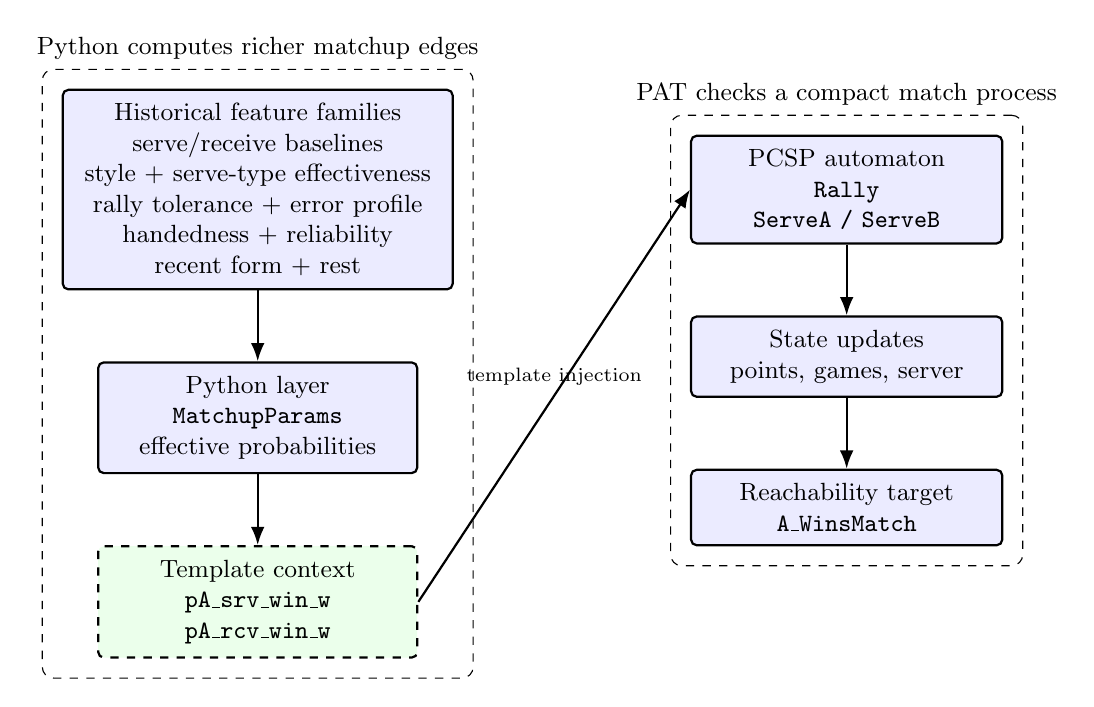
\begin{tikzpicture}[
  node distance=9mm and 10mm,
  every node/.style={font=\small}
]
\node[processbox, text width=4.6cm] (feat) {Historical feature families\\serve/receive baselines\\style + serve-type effectiveness\\rally tolerance + error profile\\handedness + reliability\\recent form + rest};
\node[processbox, below=of feat, text width=3.7cm] (matchup) {Python layer\\\texttt{MatchupParams}\\effective probabilities};
\node[artifactbox, below=of matchup, text width=3.7cm] (weights) {Template context\\\texttt{pA\_srv\_win\_w}\\\texttt{pA\_rcv\_win\_w}};

\node[processbox, right=30mm of feat, text width=3.6cm] (rally) {PCSP automaton\\\texttt{Rally}\\\texttt{ServeA / ServeB}};
\node[processbox, below=of rally, text width=3.6cm] (update) {State updates\\points, games, server};
\node[processbox, below=of update, text width=3.6cm] (reach) {Reachability target\\\texttt{A\_WinsMatch}};

\draw[flow] (feat) -- (matchup);
\draw[flow] (matchup) -- (weights);
\draw[flow] (rally) -- (update);
\draw[flow] (update) -- (reach);
\draw[flow] (weights.east) -- node[above, font=\scriptsize] {template injection} (rally.west);

\node[groupbox, fit=(feat)(matchup)(weights), label={[font=\small]north:Python computes richer matchup edges}] {};
\node[groupbox, fit=(rally)(update)(reach), label={[font=\small]north:PAT checks a compact match process}] {};
\end{tikzpicture}
}
\caption{What PAT checks versus what Python computes upstream before rendering the formal model.}
\label{fig:formal_vs_python}
\end{figure}

\subsection*{Current Matchup Parameterization Beyond Serve/Receive Baselines}
Although the checked-in PCSP\# graph is compact, the current parameterization layer is substantially richer than a plain two-parameter lookup. In the present codebase, \texttt{MatchupParams} combines baseline serve and receive strength, serve and rally-style differentials, error profile, return pressure, clutch, serve-type effectiveness, rally tolerance, stroke profile, handedness, reliability, recent form, and rest. Baseline phase probabilities are themselves blended in a reliability-aware manner using both player \(A\)'s own phase record and the complement of player \(B\)'s corresponding phase strength. Influence weights are then fit by ridge-regularized regression on pre-match historical snapshots, which reduces same-match leakage and dampens small-sample instability.

In other words, the formal model exposed to PAT remains small, but the numerical inputs to that model are calibrated from a multi-factor historical representation. This is why the repository should be understood as a compact probabilistic model checker fed by a richer statistical front-end, rather than as a hand-tuned two-number model.

\subsection*{How the Feature Families Influence Serve and Receive}
The code is also structured in a way that supports a more nuanced interpretation of the feature families than a flat list of variables might suggest. The serve and receive baselines form the starting point, but they are not used in isolation. The baseline itself is first blended from two perspectives: player \(A\)'s own observed phase strength and the complement of player \(B\)'s opposing phase strength. This means that player \(A\)'s estimated serve quality is not just ``how often \(A\) wins on serve,'' but a compromise between that quantity and ``how often \(B\) fails to win on receive,'' with both sides weighted by reliability.

On top of that baseline, the code adds two qualitatively different types of adjustments. The first type consists of broad matchup-style differentials such as short-serve mix, attacking rally share, and safe-play bias. These are the coarse tactical identity signals. The second type consists of micro-edge features such as unforced-error differential, return-pressure differential, clutch differential, serve-type effectiveness, rally tolerance, terminal error profile, handedness asymmetry, backhand usage, around-the-head usage, recent form, and rest. These are closer to matchup refinements than to top-level strategic style.

The serve and receive channels then treat these inputs differently. Return pressure is weighted more strongly on receive than on serve, because it is closer to a direct receive-side capability. Serve-type effectiveness contributes more on serve than on receive, because it is more naturally associated with the side initiating the rally. Rally tolerance, error profile, and stroke-profile features are similarly given phase-specific coefficients rather than being applied identically across both channels. This is a technically meaningful choice: the code is encoding the intuition that the same empirical signal can manifest differently depending on whether the player is serving or receiving.

Finally, the strategy-adjustment interface in \texttt{with\_adjustments()} shows how these variables are intended to support coaching interventions. Tactical advice in this repository is not generated as unrestricted prose and then post hoc justified. Instead, the code defines a limited set of adjustable levers---serve mix, attacking share, unforced-error proxy, return pressure, clutch, serve effectiveness, terminal error profile, and rally tolerance---and each of those levers changes a concrete subset of the player-\(A\) parameter object before the effective probabilities are recomputed. This gives the strategy engine an interpretable semantics: each recommendation corresponds to a bounded perturbation of specific numerical inputs, not a free-form verbal suggestion.

\begin{lstlisting}[style=code,language=Python,caption={Representative fields in the current parameter schema from \texttt{coach/model/params.py}.}]
class InfluenceWeights(BaseModel):
    w_serve_type: float = Field(default=0.03, ge=0.0, le=0.08)
    w_rally_tolerance: float = Field(default=0.02, ge=0.0, le=0.08)
    w_error_profile: float = Field(default=0.03, ge=0.0, le=0.08)
    w_handedness: float = Field(default=0.01, ge=0.0, le=0.08)
    w_backhand: float = Field(default=0.01, ge=0.0, le=0.08)
    w_aroundhead: float = Field(default=0.01, ge=0.0, le=0.08)
    w_recent_form: float = Field(default=0.06, ge=0.0, le=0.12)
    w_rest: float = Field(default=0.03, ge=0.0, le=0.1)

class PlayerParams(BaseModel):
    short_serve_skill: float = Field(default=0.5, ge=0.01, le=0.99)
    long_serve_skill: float = Field(default=0.5, ge=0.01, le=0.99)
    rally_tolerance: float = Field(default=0.5, ge=0.01, le=0.99)
    net_error_rate: float = Field(default=0.0, ge=0.0, le=1.0)
    out_error_rate: float = Field(default=0.0, ge=0.0, le=1.0)
    backhand_rate: float = Field(default=0.0, ge=0.0, le=1.0)
    aroundhead_rate: float = Field(default=0.0, ge=0.0, le=1.0)
    handedness_flag: float = Field(default=0.0, ge=0.0, le=1.0)
    reliability: float = Field(default=1.0, ge=0.0, le=1.0)
    recent_form: float = Field(default=0.5, ge=0.01, le=0.99)
    rest_days: float = Field(default=7.0, ge=0.0, le=90.0)
\end{lstlisting}

\section{Part B: The Prediction Agent (Reachability Analysis)}
Prediction queries are routed through the reachability pipeline. In the current implementation, a question such as ``What is the expected winning percentage for Viktor Axelsen vs Kento Momota?'' is handled by a plan whose semantics are: resolve players, load recent historical data, build a rendered PCSP\# model, run PAT, and summarize only the returned probability.

The data mapping stage is richer than a simple win-loss lookup. The local CSV adapter in \path{coach/data/adapters/local_csv.py} constructs a player-centric perspective frame from match rows, computes recency weights with a 45-day half-life, applies Laplace smoothing to serve and receive outcomes, applies Dirichlet-style smoothing to serve and rally-style mixtures, and derives several tactical proxies:
\begin{itemize}
\item \texttt{unforced\_error\_rate}: a proxy based on attack rate, flick rate, safe rate, and point loss;
\item \texttt{return\_pressure}: a clipped composite of receive win rate, attack share, and point share;
\item \texttt{clutch\_point\_win}: a close-match measure based on close-score point share and smoothed close-match win rate;
\item \texttt{short\_serve\_skill}, \texttt{long\_serve\_skill}, and \texttt{rally\_tolerance};
\item \texttt{net\_error\_rate}, \texttt{out\_error\_rate}, \texttt{backhand\_rate}, and \texttt{aroundhead\_rate};
\item \texttt{handedness\_flag} and \texttt{reliability};
\item \texttt{recent\_form} and \texttt{rest\_days}.
\end{itemize}

The final matchup object is assembled in \path{coach/data/stats_builder.py}. Head-to-head information is blended into the baseline using
\[
\texttt{blend} = \min\!\left(0.35,\; \frac{\texttt{h2h\_matches}}{\texttt{h2h\_matches}+12}\right),
\]
which prevents small-sample head-to-head data from overwhelming the player-level priors. The same layer also estimates influence weights from pre-match historical snapshots using ridge-style regularization, so the eventual serve/receive probabilities are shaped by both domain priors and data-driven calibration.

The reachability property is the same one encoded in the main template:
\[
\texttt{\#define A\_WinsMatch a\_games == GAMES\_TO\_WIN;}
\qquad
\texttt{\#assert BadmintonMatch reaches A\_WinsMatch with prob;}
\]
Hence the predicted winner is not a symbolic class label, but the player associated with the larger computed reachability probability. The auxiliary file \path{examples/minimal.pcsp} is used by \path{scripts/pat_check.py} as a smoke test to verify that PAT can successfully evaluate a minimal \texttt{reaches ... with prob} assertion before the full model is attempted.

At execution time, the service delegates PAT invocation to \path{coach/pat/runner.py}. In real mode, PAT is called with the \texttt{-pcsp} flag; in mock mode, the project uses a deterministic surrogate that reads the rendered parameters and returns a monotonic logistic score. The parser in \path{coach/pat/parser.py} is deliberately tolerant: it recognizes strings such as \texttt{Probability = 0.123}, \texttt{with prob 0.123}, and interval outputs such as \texttt{Probability [0.6125, 0.6125]}.

The key point is that the prediction pipeline produces more than a final scalar probability. For each run, the repository writes the rendered \path{matchup.pcsp} model, \path{params.json}, \path{stats.json}, PAT stdout/stderr, the PAT text output, and a summary record. The prediction is therefore reproducible and inspectable at every stage: historical inputs, parameter estimates, formal model instantiation, and final reachability output are all preserved as first-class artifacts.

\section{Part C: The Strategy Agent (Sensitivity Analysis)}
The strategy pipeline extends the prediction pipeline by repeatedly perturbing player \(A\)'s parameters, rerendering the model, and comparing the resulting reachability probability against the baseline. Importantly, the code does \emph{not} compute an analytic gradient from the PCSP\# process. Instead, it performs a discrete, finite-perturbation sensitivity search and interprets the observed
\[
\Delta P = P_{\text{candidate}} - P_{\text{baseline}}
\]
as a directional coaching signal. This is best understood as a gradient-like search, not symbolic differentiation.

The core search logic resides in \path{coach/service.py}. The engine defines a search space over eight tactical knobs:
\begin{itemize}
\item short-serve share,
\item attacking rally share,
\item unforced-error proxy,
\item return pressure,
\item clutch-point win rate,
\item serve-effectiveness proxy,
\item terminal error profile,
\item rally tolerance.
\end{itemize}
Single-knob moves and selected pairwise combinations are generated, deduplicated, and filtered by an \(L_1\) realism bound so that recommendations remain local rather than implausibly extreme.

It is also useful to state explicitly what the strategy engine is \emph{not} doing. PAT is not exploring a higher-order strategy-state automaton in which tactical choices are encoded as dynamic formal states. Instead, the strategy layer perturbs player-\(A\) parameters externally, re-renders a concrete \path{matchup.pcsp} instance for each candidate, and then asks PAT to evaluate those instantiated models. The search is therefore over a bounded neighborhood of parameter configurations, not over symbolic tactical policies inside the checked state machine.

\begin{lstlisting}[style=code,language=Python,caption={Fine-grained candidate generation in \texttt{coach/service.py}.}]
knob_steps: dict[str, list[float]] = {
    "serve_short_delta": [-0.08, -0.05, -0.03, -0.02, -0.01, 0.01, 0.02, 0.03, 0.05, 0.08],
    "attack_delta": [-0.08, -0.05, -0.03, -0.02, -0.01, 0.01, 0.02, 0.03, 0.05, 0.08],
    "unforced_error_delta": [-0.06, -0.04, -0.03, -0.02, -0.01, 0.01, 0.02, 0.03, 0.04, 0.06],
    "return_pressure_delta": [-0.06, -0.04, -0.03, -0.02, -0.01, 0.01, 0.02, 0.03, 0.04, 0.06],
    "clutch_delta": [-0.04, -0.03, -0.02, -0.01, 0.01, 0.02, 0.03, 0.04],
    "serve_effectiveness_delta": [-0.04, -0.03, -0.02, -0.01, 0.01, 0.02, 0.03, 0.04],
    "error_profile_delta": [-0.04, -0.03, -0.02, -0.01, 0.01, 0.02, 0.03, 0.04],
    "rally_tolerance_delta": [-0.04, -0.03, -0.02, -0.01, 0.01, 0.02, 0.03, 0.04],
}
pair_knobs = [
    ("serve_short_delta", "attack_delta"),
    ("serve_short_delta", "unforced_error_delta"),
    ("serve_short_delta", "return_pressure_delta"),
    ("attack_delta", "unforced_error_delta"),
    ("attack_delta", "clutch_delta"),
    ("return_pressure_delta", "clutch_delta"),
    ("serve_effectiveness_delta", "error_profile_delta"),
    ("serve_effectiveness_delta", "rally_tolerance_delta"),
    ("error_profile_delta", "rally_tolerance_delta"),
]
\end{lstlisting}

A second engineering choice makes the optimization computationally tractable: when the raw candidate set exceeds the search budget, the engine first scores candidates with a cheap surrogate, \texttt{mock\_probability(params.to\_template\_context())}, and only then evaluates the top-\(k\) candidates with the full PAT interface. This pre-ranking step does not replace PAT; rather, it acts as a budget-preserving filter before exact re-evaluation.

\begin{lstlisting}[style=code,language=Python,caption={Budget pruning before exact PAT re-evaluation in \texttt{coach/service.py}.}]
prepared: list[tuple[float, float, StrategyAdjustment, MatchupParams]] = []
for candidate in candidates:
    adjusted = candidate.apply_to(baseline)
    prepared.append(
        (
            self._estimate_candidate_probability(adjusted),
            adjusted.l1_change_from(baseline),
            candidate,
            adjusted,
        )
    )

prepared.sort(key=lambda item: (-item[0], item[1]))
return [(candidate, adjusted) for _, _, candidate, adjusted in prepared[:limit]]
\end{lstlisting}

Rather than hardcoding a single reproduced branch-specific strategy result into the paper, the more accurate claim is procedural: the engine generates a local set of feasible candidates, ranks them under a bounded search budget, reruns PAT on the top candidates, and returns both the best adjustment and a ranked list of alternatives. The system therefore does not say ``be more aggressive'' merely because the phrase sounds plausible. It says, in effect: \emph{within a bounded neighborhood of the estimated parameter state, these controlled perturbations produce the largest positive change in reachability probability.} The natural-language advice is therefore the final layer of a quantitative sensitivity analysis.

\section{Technical Implementation Details}
\subsection*{Glue Code and Interface Layer}
The orchestration logic is centralized in \path{coach/service.py}. The classes \texttt{PATExecution}, \texttt{PredictionResult}, \texttt{StrategyCandidate}, and \texttt{StrategyResult} provide typed payloads for every major pipeline stage. \path{main.py} simply delegates to \path{coach/cli.py}. This gives the project multiple entry points while preserving a single authoritative service layer.

\subsection*{Service Surfaces and Deployment Interfaces}
The repository currently exposes a richer deployment surface than a single command-line tool. The CLI entry points include \texttt{coach predict}, \texttt{coach strategy}, \texttt{coach pat-run}, \texttt{coach chat}, \texttt{coach experiments}, and the dedicated backtesting entry point \texttt{coach-backtest}. On the HTTP side, \path{coach/ui/app.py} exposes a FastAPI application with a landing page, a player-list endpoint, prediction and strategy endpoints, and a chat endpoint that delegates to the same typed planning/execution stack.

\begin{lstlisting}[style=code,language=Python,caption={Current FastAPI route surface in \texttt{coach/ui/app.py}.}]
@app.get("/", response_class=HTMLResponse)
@app.get("/players")
@app.post("/predict")
@app.post("/strategy")
@app.post("/chat")
\end{lstlisting}

Deployment configuration is environment-driven through \path{coach/config.py}. PAT execution is controlled by \texttt{PAT\_CONSOLE\_PATH}, \texttt{PAT\_USE\_MONO}, \texttt{MONO\_PATH}, \texttt{PAT\_TIMEOUT\_S}, and \texttt{RUNS\_DIR}. LLM integration is optional: if Gemini credentials are not present, the planner falls back to deterministic heuristic planning. When Upstash Redis is configured, the Gemini client can rotate keys globally across processes after quota errors, which gives the system a practical multi-process deployment path beyond local experimentation.

\subsection*{Interactive User Experience Layer}
The user interface layer is intentionally thin. The browser landing page served at \texttt{GET /} is a convenience shell over the same typed backend used by the CLI, not a separate inference path. \texttt{GET /players} exposes the local player registry for autocomplete and validation, while \texttt{POST /predict} and \texttt{POST /strategy} accept structured request payloads that map directly to the service layer. The chat endpoint, \texttt{POST /chat}, shares the same deterministic execution pipeline after planning, so the web experience does not bypass the underlying constraints on player resolution, model building, or PAT execution. This is an important architectural property: the interface is flexible, but the numerically decisive backend remains the same across surfaces.

\subsection*{Prompt Engineering and LLM API Usage}
Prompt engineering is deliberately restrictive. The core instructions in \path{coach/agent/prompts.py} forbid numerical guessing and require tool-based reasoning. The Gemini wrapper in \path{coach/agent/llm\_client.py} uses temperature \(0.0\) for planning and \(0.2\) for summarization, and it parses responses as strict JSON whenever a plan is requested. Crucially, the planner is optional rather than mandatory: if no working Gemini client is available, the repository still produces structured plans through a deterministic fallback path in \path{coach/agent/planner.py}. This means the repository remains operable without online LLM access.

\begin{lstlisting}[style=code,language=Python,caption={Prompt-engineering rules in \texttt{coach/agent/prompts.py}.}]
SYSTEM_PROMPT = """You are the AI Badminton Coach planner.
You must never guess probabilities. You must use tool outputs.
Rules:
1. For prediction questions, always generate tool calls that resolve players, load stats, build a PCSP model, and run PAT.
2. For strategy questions, always include a sensitivity/optimization tool call and report quantified deltas.
3. Return strict JSON only.
4. If players are ambiguous, ask to resolve via ResolvePlayers tool first.
"""

def planner_prompt(user_query: str) -> str:
    return (
        "Produce a JSON plan with keys: task_type, analysis_type, players, constraints, tool_calls. "
        f"User query: {user_query}"
    )

def summary_prompt(question: str, computed_payload: dict) -> str:
    return (
        "Use only computed outputs. Do not invent numbers. "
        "Provide concise badminton coaching advice with quantified probabilities/deltas.\n"
        f"Question: {question}\n"
        f"Computed payload: {computed_payload}"
    )
\end{lstlisting}

A further operational feature is the Redis-backed Gemini key queue. If Upstash Redis is configured, \texttt{LLMClient} rotates API keys globally across processes on quota errors such as HTTP 429 or 503. The scripts \path{scripts/seed\_redis\_keys.py}, \path{scripts/get\_redis\_keys.py}, \path{scripts/validate\_redis\_head.py}, \path{scripts/test\_redis\_rotation.py}, and \path{scripts/test\_llm\_client.py} support this deployment workflow.

\subsection*{PAT Wrapper and Robust Execution}
The PAT wrapper in \path{coach/pat/runner.py} supports both mock and real execution. Real execution resolves either a PAT executable path or a PAT installation directory, auto-detects whether Mono is required, writes stdout/stderr artifacts, and records structured metadata in \path{pat\_run.json}.

\begin{lstlisting}[style=code,language=Python,caption={Command construction for real PAT execution in \texttt{coach/pat/runner.py}.}]
def _build_pat_command(
    *,
    pat_console_path: Path,
    pcsp_path: Path,
    out_path: Path,
    use_mono: bool,
) -> list[str]:
    if use_mono:
        settings = CoachConfig.from_env()
        return [settings.mono_path, str(pat_console_path), "-pcsp", str(pcsp_path), str(out_path)]
    return [str(pat_console_path), "-pcsp", str(pcsp_path), str(out_path)]
\end{lstlisting}

A particularly notable engineering feature is PAT3-on-Mono compatibility handling. When PAT3 produces the known NESC startup failure signature, the runner clones the PAT runtime into a run-local directory, writes a small C\# shim (\texttt{nesc\_shim.cs}), compiles it with \texttt{mcs}, and retries execution. This is a strong example of repository-specific glue code: the project is not merely calling an external executable, but also repairing a real interoperability problem between PAT3 and Mono.

The mock verifier in \path{coach/pat/mock\_pat.py} is equally important. It preserves monotonic behavior and enables CI, unit tests, and development-time experimentation without requiring a PAT installation. The repository is explicit about this separation: mock mode is an engineering surrogate, while real mode is the formal-verification path.

The mock path is also more compatibility-aware than a naive stub. It does not simply return a hardcoded probability or consume an in-memory parameter object directly. Instead, it reparses parameters from the rendered \path{.pcsp} text, normalizes case-insensitive parameter names, accepts legacy aliases such as \texttt{ue\_rate\_A/B}, and then computes a deterministic logistic score from the extracted values. This makes the mock verifier useful not only for speed, but also as a robustness layer for template evolution: tests can detect mismatches between what the builder writes into the PCSP file and what downstream tooling expects to read back out.

\subsection*{Data Engineering, ETL, and Model Inputs}
The data pipeline is implemented in \path{scripts/build\_real\_data.py} and configured by \path{scripts/shuttleset\_config.py}. These files translate ShuttleSet stroke-level logs into the shipped \path{coach/data/sample\_players.csv} and \path{coach/data/sample\_matches.csv}. Chinese shot labels are mapped to English, then to tactical categories \texttt{attack}, \texttt{neutral}, and \texttt{safe}. Additional enrichment computes average rally length, long-rally share, short- and long-serve effectiveness, stroke-profile rates, and terminal error rates. The ETL code also randomly swaps the \texttt{playerA/playerB} ordering so that the winner is not trivially encoded as ``side A,'' which is a sensible anti-bias choice.

\subsection*{From Raw ShuttleSet Rallies to Match-Level Tables}
The ETL pipeline is worth unpacking because it explains exactly how the repository moves from rally traces to the historical table later consumed by the model. The function \texttt{process\_set\_csv()} reads one ShuttleSet set file and groups rows by rally identifier. Within each rally, it sorts by \texttt{ball\_round}, infers rally length, identifies the initial server from the first stroke, classifies that first stroke as short or long service, and then determines the rally winner from the terminal \texttt{getpoint\_player} annotation. This lets the code accumulate per-side counts for serve rallies, serve wins, short- and long-serve samples, short- and long-serve wins, total strokes, tactical shot categories, and terminal error causes.

The next step, \texttt{process\_match()}, aggregates those set-level counts across all sets of a match. This yields match-level totals for serve opportunities, points, games won, rally-context statistics, and the enriched tactical counters. The helper functions \texttt{compute\_rates()} and \texttt{compute\_enriched\_rates()} then convert raw counts into deterministic rate features with explicit defaults when evidence is absent. For example, serve-type win rates default to \(0.5\) when no samples are available, while backhand and around-the-head rates default to \(0.0\) in the absence of observed positive annotations. This is not merely bookkeeping: it defines the numerical semantics of sparse observations before the later smoothing and prior-blending steps performed by the local adapter.

The side-swapping step in \texttt{build\_data()} is especially important for report-writing purposes because it is a concrete anti-leakage and anti-shortcut design decision. ShuttleSet encodes the winner on side \(A\) and the loser on side \(B\), so a naive export would let downstream models exploit positional encoding rather than badminton-relevant structure. By randomly swapping the sides with a fixed seed, the repository makes \texttt{winner\_id} the authoritative label and prevents ``playerA means winner'' from surviving as a degenerate predictive cue.

The ETL layer also enforces a more disciplined schema than many prototype sports repositories. The \texttt{validate()} routine checks player-table foreign-key integrity, serve-rate and rally-style normalization constraints, probability bounds for the enriched rates, integer constraints for serve sample counts, and basic logical conditions such as serve wins not exceeding serve rallies. That validation pass matters because the downstream pipeline assumes these invariants when computing smoothed player histories and matchup parameters. In other words, the ETL is not only feature extraction; it is also a schema contract that protects later formal-model construction from malformed historical inputs.

The schema is documented in \path{coach/data/schema.md}, while \path{coach/data/adapters/web\_source.py} provides a placeholder disk-cached adapter for future web integration. The current project, however, is intentionally local-first: the operative adapter is \texttt{LocalCSVAdapter}.

Figure~\ref{fig:data_pipeline} summarizes that transformation path at the right level of abstraction for the report. It starts from rally/stroke logs, passes through deterministic ETL and schema validation, and ends only after the adapter has converted match-level tables into player-history features and PAT-ready weights. The point of the figure is to show that the shipped CSVs are an intermediate contract, not the final inferential representation.

\begin{figure}[H]
\centering
\resizebox{\linewidth}{!}{%
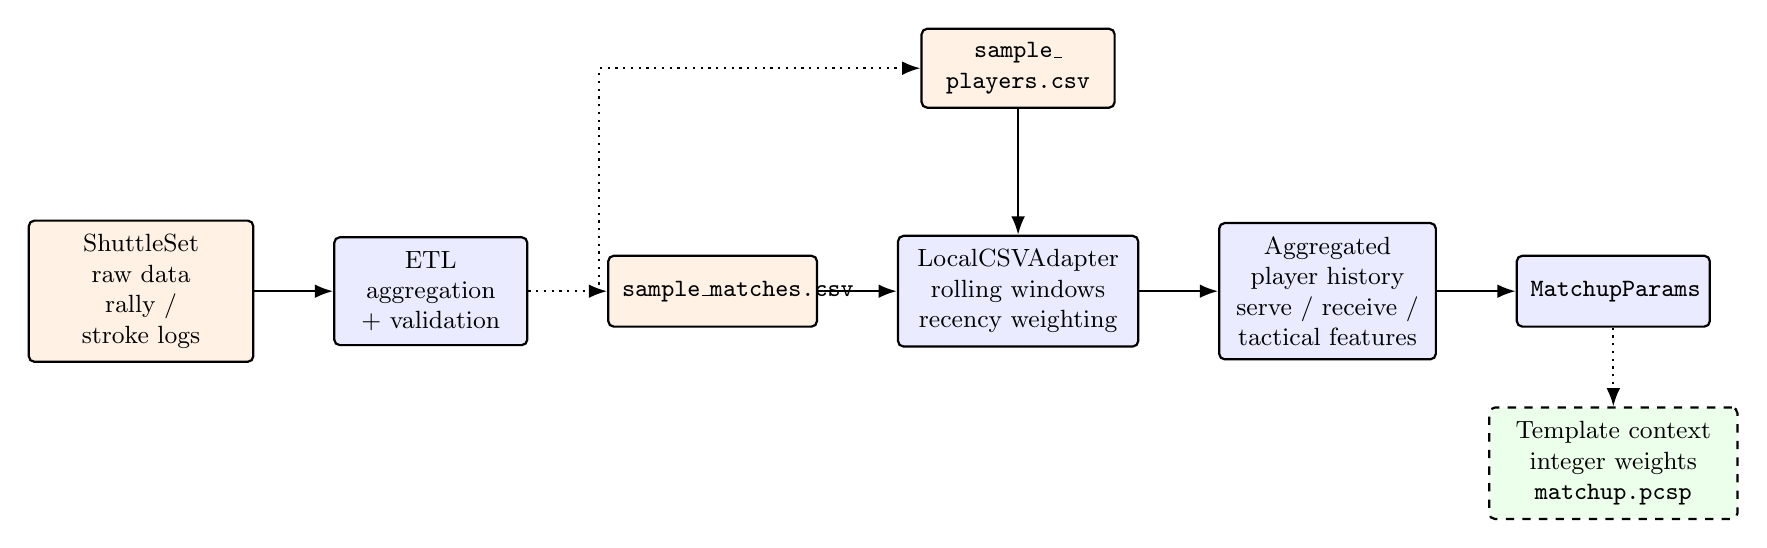
\begin{tikzpicture}[
  node distance=10mm and 10mm,
  every node/.style={font=\small}
]
\node[storebox, text width=2.5cm] (raw) {ShuttleSet raw data\\rally / stroke logs};
\node[processbox, right=of raw, text width=2.1cm] (etl) {ETL\\aggregation + validation};
\node[storebox, right=of etl, text width=2.3cm] (matches) {\texttt{sample\_matches.csv}};
\node[processbox, right=of matches, text width=2.7cm] (adapter) {LocalCSVAdapter\\rolling windows\\recency weighting};
\node[storebox, above=16mm of adapter, text width=2.1cm] (players) {\texttt{sample\_}\\\texttt{players.csv}};
\node[processbox, right=of adapter, text width=2.4cm] (features) {Aggregated player history\\serve / receive / tactical features};
\node[processbox, right=of features, text width=2.1cm] (params2) {\texttt{MatchupParams}};
\node[artifactbox, below=of params2, text width=2.8cm] (context) {Template context\\integer weights\\\texttt{matchup.pcsp}};

\draw[flow] (raw) -- (etl);
\draw[genflow] (etl) -- (matches);
\draw[genflow] (etl.east) -- ++(0.9,0) |- (players.west);
\draw[flow] (players) -- (adapter);
\draw[flow] (matches) -- (adapter);
\draw[flow] (adapter) -- (features);
\draw[flow] (features) -- (params2);
\draw[genflow] (params2) -- (context);
\end{tikzpicture}
}
\caption{Data pipeline from ShuttleSet rally logs to aggregated player-history features and PAT-ready model inputs.}
\label{fig:data_pipeline}
\end{figure}

\subsection*{Schema-Enriched Match Features}
The current \path{sample\_matches.csv} schema is more informative than a minimal serve/receive log. In addition to serve counts, points, and style mixtures, the ETL now preserves match metadata and several tactical/context features that are later aggregated into player-history statistics by the local adapter.

\begin{table}[H]
\centering
\small
\begin{tabular}{L{0.22\linewidth}L{0.70\linewidth}}
\toprule
Feature group & Current columns in \path{sample\_matches.csv} \\
\midrule
Metadata & \texttt{tournament}, \texttt{round}, \texttt{duration\_min}, \texttt{match\_sets} \\
Rally context & \texttt{avg\_rally\_len}, \texttt{long\_rally\_share} \\
Serve-type effectiveness & \texttt{a/b\_short\_serve\_win\_rate}, \texttt{a/b\_long\_serve\_win\_rate}, \texttt{a/b\_short\_serve\_samples}, \texttt{a/b\_long\_serve\_samples} \\
Stroke profile & \texttt{a/b\_backhand\_rate}, \texttt{a/b\_aroundhead\_rate} \\
Terminal error profile & \texttt{a/b\_net\_error\_lost\_rate}, \texttt{a/b\_out\_error\_lost\_rate} \\
\bottomrule
\end{tabular}
\end{table}

These are still match-level aggregates rather than raw rally-state traces, but they substantially improve the descriptive power of the historical record. The adapter later converts them into player-centric features such as \texttt{short\_serve\_skill}, \texttt{rally\_tolerance}, and stroke-profile or terminal-error metrics over a rolling historical window.

\subsection*{Reproducibility and Audit Artifacts}
Every prediction, strategy, direct PAT run, and backtest writes an auditable run directory under \path{runs/<run\_id>/}. These directories are not incidental logs; they are part of the design of the system. They preserve the exact inputs, intermediate parameter state, rendered PCSP\# model, PAT outputs, and final summaries needed to inspect or reproduce a run.

\begin{table}[H]
\centering
\small
\begin{tabular}{L{0.24\linewidth}L{0.66\linewidth}}
\toprule
Artifact & Purpose \\
\midrule
\path{inputs.json} & Records task type, players, mode, window, and run metadata. \\
\path{stats.json} & Stores player-level historical statistics, head-to-head data, and fitted weights. \\
\path{params.json} & Stores validated \texttt{MatchupParams}, exported template context, and effective probabilities. \\
\path{prediction\_result.json} / \path{strategy\_result.json} & Stores the structured result payload returned by the service layer. \\
\path{summary.json} & Stores the concise end-user summary and core probability outputs. \\
Rendered \path{.pcsp} files & Preserve the exact formal model sent to PAT. \\
\path{pat\_stdout.txt}, \path{pat\_stderr.txt}, \path{pat\_output.txt}, \path{pat\_run.json} & Preserve PAT execution traces, parsed outputs, and command metadata. \\
\path{top\_alternatives.csv} & Stores ranked strategy alternatives for sensitivity runs. \\
\bottomrule
\end{tabular}
\end{table}

This artifact trail is a central strength of the repository. The project is not only producing a final answer; it is preserving the exact intermediate model and parameter state needed for later inspection, debugging, and empirical comparison.

A further repository-specific detail is that \path{pat\_run.json} is richer than a generic ``subprocess log.'' In real PAT mode, the runner records whether fallback logic was applied, preserves per-attempt command metadata, and stores enough information to reconstruct multi-step execution behavior rather than only the final return code. If PAT3-on-Mono compatibility handling is triggered, the run directory may additionally contain \path{pat\_stdout\_attempt1.txt}, \path{pat\_stderr\_attempt1.txt}, later-attempt logs, and shim-compilation files such as \path{pat3\_shim\_compile\_stdout.txt}, \path{pat3\_shim\_compile\_stderr.txt}, and \path{pat3\_shim\_compile\_cmd.txt}. This means the repository supports not only scientific reproducibility of probabilities, but also forensic reproducibility of solver invocation and recovery behavior.

It is also worth noting that \path{summary.json} exists at two levels of abstraction. The low-level PAT runner writes a minimal summary containing essentially the parsed probability, while the higher-level service later overwrites that file with a richer task-oriented summary containing players, the question type, and the parameters used. This layered artifact behavior is subtle but meaningful: the codebase preserves both solver-level and application-level perspectives on a run, even though they share a common summary filename within service-managed directories.

\subsection*{Minimal Reproduction Workflow}
The repository is also straightforward to exercise from the command line. A minimal prediction run can be reproduced with \texttt{coach predict --a "Viktor Axelsen" --b "Kento Momota" --mode mock}, while a sensitivity run can be reproduced with \texttt{coach strategy --a "Viktor Axelsen" --b "Kento Momota" --mode mock}. Leakage-aware evaluation can be reproduced with \texttt{coach-backtest run --mode mock}. If PAT is installed and configured through \texttt{PAT\_CONSOLE\_PATH}, the same commands can be rerun with \texttt{--mode real}. The most useful files to inspect after prediction or strategy are the rendered \path{matchup.pcsp}, \path{params.json}, \path{stats.json}, and \path{summary.json}; after backtesting, the key summary artifact is \path{metrics.json}, supplemented by CSV outputs for predictions, skipped cases, and calibration summaries.

\begin{lstlisting}[style=code,language=bash,caption={Minimal reproduction commands for prediction, strategy, and backtesting.}]
coach predict --a "Viktor Axelsen" --b "Kento Momota" --mode mock
coach strategy --a "Viktor Axelsen" --b "Kento Momota" --mode mock
coach-backtest run --mode mock

# Optional if PAT is installed and configured
coach predict --a "Viktor Axelsen" --b "Kento Momota" --mode real
coach strategy --a "Viktor Axelsen" --b "Kento Momota" --mode real
\end{lstlisting}

\subsection*{A Single-Run Audit Trail}
Figure~\ref{fig:audit_trail} gives the same idea in artifact form rather than as an API pipeline. It shows what is persisted at each stage of one prediction run and why the run directory is useful both for scientific reproducibility and for debugging. The figure deliberately stays at the file-contract level, because the detailed meaning of each artifact is already explained in the surrounding prose and tables.

\begin{figure}[H]
\centering
\resizebox{\linewidth}{!}{%
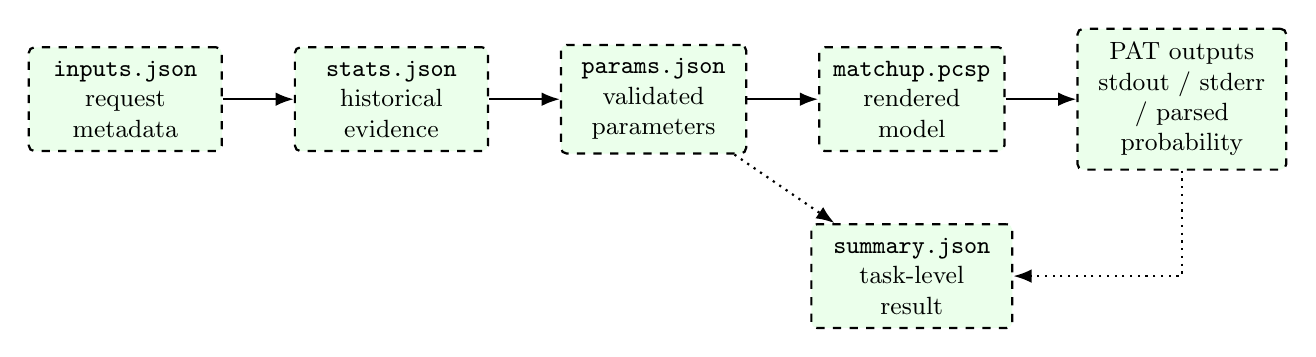
\begin{tikzpicture}[
  node distance=9mm and 9mm,
  every node/.style={font=\small}
]
\node[artifactbox, text width=2.1cm] (inputs) {\texttt{inputs.json}\\request metadata};
\node[artifactbox, right=of inputs, text width=2.1cm] (stats) {\texttt{stats.json}\\historical evidence};
\node[artifactbox, right=of stats, text width=2.0cm] (params3) {\texttt{params.json}\\validated parameters};
\node[artifactbox, right=of params3, text width=2.0cm] (pcsp2) {\texttt{matchup.pcsp}\\rendered model};
\node[artifactbox, right=of pcsp2, text width=2.3cm] (patout) {PAT outputs\\stdout / stderr / parsed probability};
\node[artifactbox, below=of pcsp2, text width=2.2cm] (summary) {\texttt{summary.json}\\task-level result};

\draw[flow] (inputs) -- (stats);
\draw[flow] (stats) -- (params3);
\draw[flow] (params3) -- (pcsp2);
\draw[flow] (pcsp2) -- (patout);
\draw[genflow] (patout) |- (summary);
\draw[genflow] (params3) -- (summary);
\end{tikzpicture}
}
\caption{Artifact trail of a single prediction run, from request metadata through rendered model and solver outputs to task-level summary.}
\label{fig:audit_trail}
\end{figure}

One useful way to understand the system is to follow a single prediction run as an audit trail rather than as an opaque API call. A run begins with player resolution against the local registry, after which the adapter assembles player-centric historical frames and derives recent-form, serve, receive, style, and tactical proxy features. These statistics are then converted into validated \texttt{MatchupParams}, exported to \path{params.json}, and rendered into a concrete \path{matchup.pcsp} instance. PAT or the mock verifier is then executed against that rendered model, and the resulting probability is written alongside the original historical statistics in \path{stats.json}, the parsed PAT output, and a concise \path{summary.json}. The important point is not a single branch-specific number, but that the repository makes every stage of the computational path visible and inspectable after the run completes.

The same audit perspective is useful for failure analysis. If a PAT run fails, the first files to inspect are \path{pat\_stdout.txt}, \path{pat\_stderr.txt}, and \path{pat\_run.json}; together they reveal whether the failure was due to a model parse issue, an empty PAT output, an execution timeout, or a PAT3-on-Mono startup incompatibility. If the run involved compatibility fallback, the attempt-specific logs and shim-compilation artifacts make it possible to distinguish ``the original PAT call failed but the fallback succeeded'' from ``both the primary and fallback paths failed.'' For strategy runs, \path{top\_alternatives.csv} and the candidate directories additionally reveal whether the best recommendation was unique or emerged from a cluster of similarly good local perturbations. This makes the run directory usable not only as a proof of execution, but also as an explanatory object for debugging, teaching, and model-forensics work.

\subsection*{Experimental Support, Backtesting, and Validation}
The files \path{coach/analysis/batch\_predict.py}, \path{coach/analysis/batch\_strategy.py}, \path{coach/analysis/experiments.py}, and \path{coach/analysis/plots.py} provide reproducible experiment runners and static plots. The plotting code uses a headless Matplotlib backend and writes artifacts under the run directory.

The most research-relevant evaluation code is in \path{coach/backtest}. \texttt{TimeMachineBacktester} builds point-in-time snapshot adapters, scores matches chronologically, compares the PCSP model against an Elo baseline and an online recent-form logistic model, and applies a rolling Platt calibrator. The feature-contract generator in \path{coach/backtest/feature\_contract.py} is especially valuable because it turns the implicit feature set into an explicit specification, including raw columns, computations, and inference requirements.

\begin{table}[H]
\centering
\small
\begin{tabular}{L{0.24\linewidth}L{0.62\linewidth}}
\toprule
Evaluation component & Role \\
\midrule
PCSP model & Main reachability-based prediction pipeline under PAT or mock execution. \\
Elo baseline & Lightweight rating baseline for comparative evaluation. \\
Recent-form logistic model & Online learned baseline over a compact feature vector derived from matchup parameters. \\
Rolling Platt calibrator & Probability calibration layer applied across models in walk-forward evaluation. \\
\bottomrule
\end{tabular}
\end{table}

Rather than relying on a single one-off score, the backtesting stack is designed to evaluate the repository chronologically under explicit leakage controls. This makes the evaluation story more compelling than a simple interactive demo, even when some experiments are run in mock mode for engineering convenience.

Figure~\ref{fig:walk_forward_loop} gives the evaluation loop a timeline view. The abstraction is chronological rather than architectural: the figure is meant to show what information is available at each scoring step, when calibration updates happen, and where skipped matches fit into the workflow. This is the clearest visual way to communicate why the backtester is leakage-aware rather than just historically trained.

\begin{figure}[H]
\centering
\resizebox{\linewidth}{!}{%
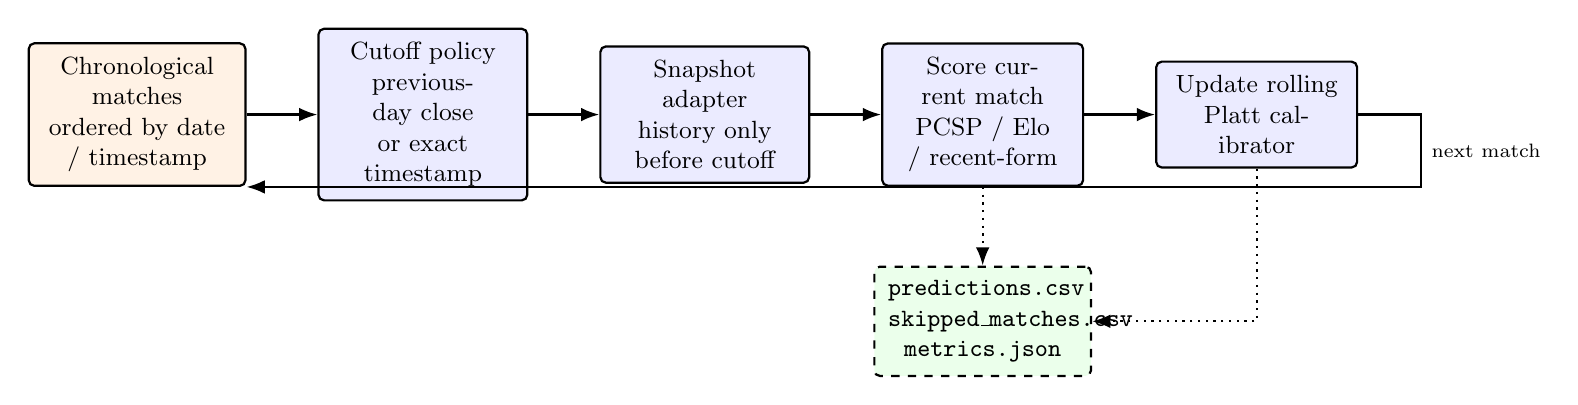
\begin{tikzpicture}[
  node distance=10mm and 9mm,
  every node/.style={font=\small}
]
\node[storebox, text width=2.4cm] (matches2) {Chronological matches\\ordered by date / timestamp};
\node[processbox, right=of matches2, text width=2.3cm] (cutoff) {Cutoff policy\\previous-day close\\or exact timestamp};
\node[processbox, right=of cutoff, text width=2.3cm] (snapshot) {Snapshot adapter\\history only before cutoff};
\node[processbox, right=of snapshot, text width=2.2cm] (score) {Score current match\\PCSP / Elo / recent-form};
\node[processbox, right=of score, text width=2.2cm] (cal) {Update rolling\\Platt calibrator};
\node[artifactbox, below=of score, text width=2.4cm] (artifacts2) {\texttt{predictions.csv}\\\texttt{skipped\_matches.csv}\\\texttt{metrics.json}};

\draw[flow] (matches2) -- (cutoff);
\draw[flow] (cutoff) -- (snapshot);
\draw[flow] (snapshot) -- (score);
\draw[flow] (score) -- (cal);
\draw[flow] (cal.east) -- ++(0.8,0) |- node[pos=0.25, right, font=\scriptsize] {next match} (matches2.south east);
\draw[genflow] (score) -- (artifacts2);
\draw[genflow] (cal) |- (artifacts2.east);
\end{tikzpicture}
}
\caption{Walk-forward backtesting loop with point-in-time snapshots, model comparison, calibration updates, and persisted evaluation artifacts.}
\label{fig:walk_forward_loop}
\end{figure}

\subsection*{Why the Baselines Matter}
The baseline models are simple by design, and that simplicity is methodologically valuable. The Elo baseline supplies a familiar rating-system comparator that updates only from prior outcomes and therefore tests whether the formal-plus-statistical pipeline is actually outperforming a standard sports-prediction heuristic. The online recent-form logistic model occupies a different role: it is not a formal-methods baseline, but a lightweight learned model over a compact feature vector derived from the same matchup-parameter space. Its feature vector includes serve and receive baseline differentials, recent form, rest, unforced-error differential, return pressure, clutch, serve skill, rally-style asymmetries, and stroke-profile asymmetries. This makes it a useful ``same information family, simpler model class'' comparator against the PCSP pipeline.

The rolling Platt calibrator then adds a third layer of methodological interest. Rather than fitting one calibration map on the full dataset and retrospectively correcting all probabilities, the repository updates a bounded rolling history online. Before the minimum sample threshold is reached, probabilities are left unchanged; after enough evidence accumulates, the calibrator learns a logistic map on the logit-transformed raw probabilities. This is a stronger walk-forward protocol than post hoc global calibration because it preserves temporal realism: at each evaluation step, calibration is based only on prior forecast-outcome pairs.

\subsection*{Evaluation Methodology}
The evaluation protocol is walk-forward and chronological rather than based on a random train/test split. \texttt{TimeMachineBacktester} first prepares matches in date order, then constructs a point-in-time snapshot adapter for each match cutoff so that every scored prediction uses only information available before that match. This is a more faithful protocol for sports forecasting than random shuffling because it preserves the temporal structure of form, rest, and accumulated evidence. The repository also tracks coverage explicitly: some matches are scored, while others may be skipped if the historical basis is insufficient or a run fails, and both outcomes are written to separate artifacts. Finally, the comparison across three models---PCSP, Elo, and recent-form logistic---is methodologically useful because it distinguishes the value of the full formal-plus-statistical pipeline from simpler rating and online-learning baselines.

Another useful detail is that the backtester caches snapshot adapters by cutoff key. This does not change the semantics of the experiment, but it does matter for reproducibility and efficiency: repeated accesses to the same historical cutoff reuse a frozen in-memory view rather than rebuilding it from scratch. The resulting workflow is closer to a sequence of point-in-time database snapshots than to repeatedly mutating one global table. In a small repository this may seem like an implementation nicety, but it supports the broader claim that the evaluation code was designed to respect temporal state explicitly rather than only approximate it informally.

\subsection*{Calibration, Coverage, and Comparative Metrics}
The backtesting outputs distinguish between raw and calibrated probabilities. For each model, the repository records accuracy-style metrics such as accuracy, precision, and recall, but it also records log loss and calibration summaries in \path{metrics.json}. This distinction matters because a forecasting system can classify winners reasonably well while still being poorly calibrated as a probability forecaster. The reported expected calibration error measures how closely forecast bins align with observed win frequencies, while textual calibration summaries provide a more interpretable description of over- or under-confidence. Coverage is reported separately from accuracy because a model that scores only easy cases is not directly comparable to a model that covers the full chronological stream. The result is a more complete evaluation frame: classification quality, probabilistic quality, and match-coverage behavior are treated as different axes of performance rather than collapsed into a single number.

The metric implementation also reflects a sensible division between decision quality and probability quality. Accuracy, precision, and recall are computed after thresholding at \(0.5\), which is appropriate for winner prediction. Log loss instead evaluates the full probability assignment and penalizes confident mistakes more heavily than hesitant ones. Calibration tables then bin probabilities and compare mean forecast to empirical win rate, while expected calibration error aggregates the absolute gaps weighted by bin support. This layered metric design is stronger than a single-score evaluation because it can reveal different failure modes: a model may rank outcomes well but be miscalibrated, or it may be well calibrated but weakly discriminative, and the repository's outputs are structured to expose those distinctions.

\begin{table}[H]
\centering
\small
\begin{tabular}{L{0.24\linewidth}L{0.62\linewidth}}
\toprule
Metric family & Interpretation \\
\midrule
Accuracy / precision / recall & Whether the model predicts the correct winner under a thresholded decision rule. \\
Log loss & Whether the forecast assigns high probability to outcomes that actually occur, rewarding confident correctness and penalizing confident error. \\
Calibration / expected calibration error & Whether predicted probabilities correspond to observed frequencies rather than only ranking quality. \\
Coverage / skipped-match rate & How often the evaluation pipeline can produce a valid point-in-time prediction across the chronological match stream. \\
\bottomrule
\end{tabular}
\end{table}

\subsection*{Backtest Outputs as Research Artifacts}
The backtester writes more than a scalar scoreboard. \path{predictions.csv} supports per-match error analysis, while \path{skipped\_matches.csv} makes coverage gaps auditable rather than silently dropped. \path{model\_metrics.csv} and \path{segmented\_metrics.csv} support model comparison both overall and within subsets such as round, tournament, discipline, or calendar year. \path{calibration.csv} provides the binned data needed to inspect reliability curves, and \path{metrics.json} collects the overall summary, rankings, and calibration diagnostics in a machine-readable form. The human-readable \path{summary.txt} provides a compact narrative of the same run, and \path{feature\_contract.md} captures the inference interface used by the evaluation. Taken together, these outputs make the backtesting directory a reusable research artifact rather than only a one-time console report.

The segmented outputs are especially helpful for turning the repository into a genuine analytical instrument rather than a one-number leaderboard. Because \path{segmented\_metrics.csv} can slice by round bucket, tournament, discipline, or calendar year, it becomes possible to ask whether the PCSP pipeline behaves differently in finals than in early rounds, or whether calibration quality drifts across different temporal subsets. Similarly, \path{predictions.csv} and \path{skipped\_matches.csv} allow downstream manual review of individual cases: one can inspect whether a miss came from an implausible probability, a cold-start prior, a sparse head-to-head signal, or a systematic tendency in one of the baseline models.

\begin{table}[H]
\centering
\small
\begin{tabular}{L{0.26\linewidth}L{0.60\linewidth}}
\toprule
Backtest artifact & Analytical use \\
\midrule
\path{predictions.csv} & Per-match error analysis, model comparison, and downstream plotting. \\
\path{skipped\_matches.csv} & Coverage auditing and diagnosis of cold-start or execution failures. \\
\path{model\_metrics.csv} & Overall cross-model summary metrics in tabular form. \\
\path{segmented\_metrics.csv} & Performance slicing by round, tournament, discipline, or year. \\
\path{calibration.csv} & Reliability and probability-calibration diagnostics. \\
\path{metrics.json} & Machine-readable summary including rankings and expected calibration error. \\
\path{summary.txt} & Human-readable digest of the same evaluation run. \\
\path{feature\_contract.md} & Frozen feature interface for reproducibility and future model replacement. \\
\bottomrule
\end{tabular}
\end{table}

\subsection*{Cold-Start Handling and Leakage Control}
Leakage control is one of the most important research-facing strengths of the repository and should be read as a first-class design choice rather than an implementation detail. In backtesting mode, \texttt{TimeMachineBacktester} creates point-in-time snapshot adapters so that each match is scored using only information available before the match cutoff. Historical statistics are computed strictly from pre-cutoff matches, and influence weights are fit from pre-match player-history snapshots rather than same-match labels. This sharply reduces temporal leakage in both player-level features and weight estimation.

The cutoff policy itself is more careful than a single generic ``train on the past'' statement suggests. When no explicit timestamp column is available, the evaluator uses a \texttt{previous\_day\_close} policy: the match is sorted by date and the cutoff is the prior day, which ensures that same-day matches are not accidentally visible in the historical snapshot. When an exact timestamp column is available, the evaluator switches to an \texttt{exact\_timestamp} policy and sets the snapshot cutoff to one second before the recorded match time. This allows the backtester to preserve same-day history when it truly precedes the target match, while still excluding future information at sub-day granularity. That detail makes the chronological evaluation story significantly stronger, because it shows that the code explicitly handles both coarse and fine temporal resolutions.

The codebase also distinguishes between production prediction and evaluation-oriented cold-start handling. The normal prediction path is comparatively strict: if there is no meaningful historical basis for a player, the system raises a failure rather than silently fabricating a profile. In contrast, the backtester can optionally enable cold-start fallback so that chronological evaluation can proceed on sparse early-history cases. This distinction is methodologically sensible because it preserves the honesty of live prediction while still allowing a realistic walk-forward evaluation protocol.

For engineering efficiency, the backtester also distinguishes between a \texttt{fast\_mock} path and persisted per-match formal artifacts. In \texttt{fast\_mock} mode, the evaluation loop can use the deterministic mock scorer directly from template context without materializing a full PAT artifact directory for every match. When \texttt{persist\_match\_artifacts} is enabled, however, the backtester writes per-match \path{matchup.pcsp} and PAT outputs under the run directory, which is useful for deep inspection of specific cases. This is a sensible separation between high-throughput experimentation and artifact-heavy forensic analysis.

\subsection*{Feature Contract for Inference and Evaluation}
The file \path{coach/backtest/feature\_contract.py} turns the system's implicit feature assumptions into an explicit inference contract. It enumerates template-context outputs, player-level features, weight features, source tables, raw columns, and the computation used to derive each field. This is unusually valuable for a repository of this size. It means the model is not only implemented, but also documented in a machine-readable and human-readable form that can support auditing, future model replacement, and downstream reproducibility.

The evaluation tooling is complemented by a dedicated CLI surface in \path{coach/backtest/cli.py}, which separates contract export, dataset ingestion, and chronological evaluation into distinct commands. This separation is helpful both conceptually and practically: the feature contract can be frozen independently, the historical dataset can be rebuilt when needed, and the evaluator can then be rerun under controlled conditions.

\begin{lstlisting}[style=code,language=bash,caption={Backtesting CLI surface exposed in \texttt{coach/backtest/cli.py}.}]
coach-backtest contract
coach-backtest ingest
coach-backtest run --mode mock
\end{lstlisting}

Validation is robust throughout the repository. The automated suite covers ETL enrichment, PAT parsing, PAT error signaling, model rendering, parameter constraints, end-to-end mock prediction and strategy behavior, service-level optimization logic, and time-machine backtesting. In the analyzed environment, all 66 tests passed. The support files \path{pyproject.toml}, \path{requirements.txt}, \path{pytest.ini}, \path{.ruff.toml}, \path{Makefile}, \path{.env.example}, and \path{.github/workflows/ci.yml} collectively define installation, linting, testing, PAT configuration, and CI behavior on Python 3.11 and 3.12. The repository also includes \path{README.md} and a shorter project summary in \path{REPORT.md}; the present document is a fuller academic reconstruction of the same implementation.

\section{Limitations and Threats to Validity}
Several limitations remain and should be stated explicitly. First, the shipped dataset is still very small: 27 players and 44 matches. This is sufficient for a meaningful systems case study, but it is not large enough to justify strong claims of broad statistical generalization. Second, many tactical inputs are aggregate proxies rather than true rally-state dynamics. Features such as unforced-error rate, return pressure, serve-type effectiveness, and rally tolerance are useful abstractions, but they are still compressed summaries of richer match behavior.

Third, the formal model and the upstream parameterization layer operate at different levels of detail. The checked-in PCSP\# template is intentionally simpler than the Python feature pipeline; it models a compact serve/receive match automaton rather than explicitly representing richer tactical state transitions such as stroke type, rally phase, or geometric court position. This is a defensible engineering tradeoff, but it also bounds what can be claimed about the formal model itself. Fourth, some features depend on sparse terminal-event labels such as \texttt{lose\_reason}, so they should be read as directional signals rather than exhaustive causal explanations.

Fifth, the fitted influence weights are estimated under small-sample conditions and with substantial regularization. This is a reasonable engineering choice, but it means the learned coefficients should be interpreted as stabilized heuristics rather than as high-confidence causal effect estimates. Their value is that they make the front-end parameterization adaptive and leakage-aware, not that they definitively settle the true tactical importance of every feature family in elite badminton.

Sixth, the strategy engine is deliberately local. It searches over bounded perturbations of the estimated baseline profile and ranks them under an \(L_1\) realism constraint plus a fixed evaluation budget. This is a sensible design for interpretable coaching suggestions, but it does mean the engine is not solving a globally optimal control problem over the match process. Recommendations should therefore be read as ``best local adjustments found within the explored neighborhood'' rather than as universally optimal tactical policies.

Finally, mock mode is a useful engineering surrogate for CI, development, and search-budget pruning, but it is not formal verification. Exact probability claims should therefore be tied either to reproduced real PAT runs or to clearly labeled mock-mode experiments. More generally, any hardcoded benchmark number in this repository should be treated as development-time evidence unless it is connected to a reproducible run artifact on the current branch.

\subsection*{Future Extensions}
The most obvious technical extension is to narrow the current gap between the rich statistical front-end and the compact formal back-end. A future version of the repository could represent additional explicit state inside the PCSP\# model itself, for example serve type, coarse rally phase, or a limited tactical mode variable. Doing so would move more of the current upstream numerical compilation into the formally checked transition structure, albeit at the cost of a larger process graph and heavier model-checking demands.

On the data side, the repository is well positioned for scale-up. The existing ingestion and schema-validation path could be connected to larger historical datasets or live feeds, while the placeholder web adapter could evolve into a true production data source. A larger dataset would support stronger calibration claims, more stable influence-weight fitting, and more informative segmented backtest analyses. It would also make it easier to test whether the current handcrafted tactical proxies remain useful once richer observation coverage is available.

On the optimization side, the current bounded local search could be generalized into a richer constrained optimization layer. The present engine already has the right semantics for interpretable levers, so a natural next step would be to explore adaptive search schedules, multi-objective tradeoffs, or optimization subject to explicit realism and fatigue constraints. Likewise, the current badminton-specific template suggests a broader family of sport-specific agent architectures in which an LLM remains a planner and explainer, while the numerically decisive step is delegated to a compact formal or simulation-based engine tailored to the scoring logic of the sport.

\section{Conclusion}
The codebase succeeds in building a practically useful bridge between LLM interaction and formal probabilistic reasoning. Its most important architectural decision is not merely that it ``uses an LLM'' and ``uses PAT,'' but that it assigns them sharply different epistemic roles. The LLM plans and explains; Python validates, compiles, and executes; PAT evaluates a formally stated reachability property; and the returned coaching advice is grounded in computed probabilities rather than stylistic plausibility.

Several extensions are clearly enabled by the current design. The stubbed web adapter could be replaced with live data feeds; the current badminton template could be generalized into a family of sport-specific PCSP\# models; the strategy engine could move from bounded local perturbation search toward richer constrained optimization; and future evaluations should emphasize real PAT mode at larger scale. Even in its present form, however, the repository already demonstrates a coherent research contribution: natural-language sports analysis can be made substantially more trustworthy when the numerically decisive step is transferred from a black-box language model into an explicit probabilistic model-checking workflow.

\end{document}
